\documentclass[11pt]{beamer}
\usetheme{Madrid}
\usefonttheme{serif}

\usepackage[utf8]{inputenc}
\usepackage[english]{babel}
\usepackage[T1]{fontenc}

\usepackage{amsmath}
\usepackage{amsfonts}
\usepackage{amssymb}
\usepackage{graphicx}
\usepackage{tcolorbox}
\tcbuselibrary{theorems, breakable,}
\tcbuselibrary{skins}



\colorlet{myred}{red!80!black}
\colorlet{myblue}{blue!80!black}
\colorlet{mygreen}{green!40!black}
\colorlet{mypurple}{red!50!blue!90!black!80}
\colorlet{mydarkred}{myred!80!black}
\colorlet{mydarkblue}{myblue!80!black}
\colorlet{mymagenta}{magenta}
\colorlet{xcol}{blue!60!black}
\colorlet{Defcol}{red!5}
\colorlet{Satzcol}{blue!90!black!80!cyan!10!white}
\colorlet{Korcol}{blue!10!white}
\colorlet{Axcol}{purple!10!white}
\colorlet{Bemcol}{black!2!white}
\colorlet{Motcol}{cyan!10!white}
\colorlet{Bspcol}{green!50!olive!2!white}
\colorlet{Bewcol}{yellow!5!white}

\newcounter{my}[section]
\def\themytheorem{\thesection.\arabic{my}}

\tcbset{
thmstyle/.style={enhanced, breakable, attach boxed title to top left={yshift=-0.9mm,xshift=2.5mm}, boxrule=0.15mm, boxed title style={boxrule=0.15mm}, fonttitle=\itshape\bfseries},
bewstyle/.style={skin=enhanced, parbox=false,boxrule=0.15mm,leftrule=0.5mm,rightrule=0.15mm, coltitle=black, breakable, fonttitle=\itshape},
bemstyle/.style={skin=enhanced, parbox=false,boxrule=0.15mm,leftrule=0.5mm,rightrule=0.15mm, coltitle=black, breakable, fonttitle=\itshape\bfseries},
}

 \newtcbtheorem[auto counter, number within= section]{Def}{Definition}{thmstyle,colback=Defcol,colframe=red!55!black!98!white,colbacktitle=red!75!black!30!pink}{Def}
 
\newtcbtheorem[use counter from= Def]{Satzz}{Theorem}{thmstyle,colback=Satzcol, colframe=blue!80!black!99!cyan,colbacktitle=blue!85!black!80!cyan!60!white,}{Satz}

\newtcbtheorem[use counter from= Def]{Lemmaa}{Lemma}{thmstyle,colback=Satzcol, colframe=blue!80!black!99!cyan,colbacktitle=blue!85!black!80!cyan!60!white,}{Lemma}

 \newtcbtheorem[use counter from= Def]{Prop}{Proposition}{thmstyle,colback=Satzcol, colframe=blue!80!black!99!cyan,colbacktitle=blue!85!black!80!cyan!60!white,}{Prop}
 
 \newtcbtheorem[use counter from= Def]{Kor}{Corollary}{thmstyle,colback=Korcol, colframe=blue!30!black,colbacktitle=blue!40!white}{Kor}
 
 \newtcbtheorem[use counter from= Def]{Ax}{Axiom}{thmstyle,colback=Axcol, colframe=purple!30!black,colbacktitle=purple!40!white}{Ax}
 
\newtcbtheorem[use counter from= Def]{Bemerkung}{Remark}{bemstyle,colback=Bemcol, colframe=white!30!black,colbacktitle=black!5!white}{Bem}

\newtcbtheorem[use counter from= Def]{Notation}{Notation}{bemstyle,colback=Bemcol, colframe=white!30!black,colbacktitle=white}{Notation}

\newtcbtheorem[use counter from= Def]{Motivation}{Motivation}{thmstyle,colback=Motcol, colframe=cyan!30!black,colbacktitle=cyan!40!white}{Mot}




%\newtcolorbox[use counter from= Def]{Bemerkung}{breakable, empty, coltitle=black, title=\textbf{Bemerkung.}}
%\newtbctheorem[use counter from= Def]{Bemerkung}{Bemerkung}{thmstyle,colback=cyan!10!white, colframe=cyan!30!black,colbacktitle=cyan!40!white}{Bemerkung}



\newtcolorbox{Formel}{bewstyle,colback=blue!90!black!80!cyan!10!white, colframe=blue!30!black,colbacktitle=blue!90!black!80!cyan!10!white,}

% \tcbmaketheorem{Def}{Definition}{thmstyle, colback=red!5,colframe=red!55!black!98!white,colbacktitle=red!75!black!30!pink}{my}{def}

% \tcbmaketheorem{Satz}{Satz}{thmstyle,colback=blue!90!black!80!cyan!10!white, colframe=blue!80!black!99!cyan,colbacktitle=blue!85!black!80!cyan!60!white,}{my}{thm}

% \tcbmaketheorem{Lemma}{Lemma}{thmstyle,colback=blue!90!black!80!cyan!10!white, colframe=blue!80!black!99!cyan,colbacktitle=blue!85!black!80!cyan!60!white,}{my}{lemma}

% \tcbmaketheorem{Prop}{Proposition}{thmstyle,colback=blue!90!black!80!cyan!10!white, colframe=blue!80!black!99!cyan,colbacktitle=blue!85!black!80!cyan!60!white,}{my}{prop}

% \tcbmaketheorem{Kor}{Korollar}{thmstyle,colback=blue!10!white, colframe=blue!30!black,colbacktitle=blue!40!white}{my}{kor}

% \tcbmaketheorem{Beispiel}{Beispiel}{bewstyle,colback=green!10!white!97!olive, colframe=green!65!olive,colbacktitle=green!10!white!97!olive, title=\textbf{Beispiel.}}{my}{bsp}


\DeclareMathOperator{\sen}{sen}
\DeclareMathOperator{\tg}{tg}

\setbeamertemplate{caption}[numbered]

\author[Autor]{Arianna Rast}
\title{Basis pursuit II}
\newcommand{\email}{email}
\newcommand{\CC}{\mathbb{C}}
\newcommand{\NN}{\mathbb{N}}
\newcommand{\KK}{\mathbb{K}}
\renewcommand{\emph}{\textbf}
\newcommand{\pp}{\partial}
\newcommand{\sgn}{\text{sgn}}
\newcommand{\p}[2]{\left\langle #1,#2\right\rangle}
\newcommand{\supp}{\text{supp}}
\newcommand{\I}{\mathrm{i}}
\newcommand{\e}{\mathrm{e}}
\newcommand{\RR}{\mathbb R}
\newcommand{\cone}{\mathrm{cone}}
%\setbeamercovered{transparent} 
\setbeamertemplate{navigation symbols}{} 

\institute[]{LMU Munich} 
\date{\today} 
%\subject{}

% ---------------------------------------------------------
% Selecione um estilo de referência
\bibliographystyle{apalike}

%\bibliographystyle{abbrv}
%\setbeamertemplate{bibliography item}{\insertbiblabel}
% ---------------------------------------------------------

% ---------------------------------------------------------
% Incluir os slides nos quais as referências foram citadas
%\usepackage[brazilian,hyperpageref]{backref}

%\renewcommand{\backrefpagesname}{Citado na(s) página(s):~}
%\renewcommand{\backref}{}
%\renewcommand*{\backrefalt}[4]{
%	\ifcase #1 %
%		Nenhuma citação no texto.%
%	\or
%		Citado na página #2.%
%	\else
%		Citado #1 vezes nas páginas #2.%
%	\fi}%
% ---------------------------------------------------------

\begin{document}

\begin{frame}
\titlepage
\end{frame}

\begin{frame}{Summary}
\tableofcontents 
\end{frame}

\begin{frame}{Review Exact Reconstruction}
\begin{itemize}
	\item For \(A\in \KK^{m\times N}\) and \(s\in \NN\) we have that
	\begin{align*}
	\left.\begin{array}{c}
		\forall x\in \CC^N\,s\text{-sparse}:\\
		x\text{ is the unique minimizer} \\  \text{of }
		\left\{\|z\|_1\,\big|\, Az=Ax\right\}
	\end{array}\right\}
\iff  A\text{ satisfies the NSP of order }s.
\end{align*}
\item Also, 
\[\left.\begin{array}{c}
		\forall x\in \CC^N\,s\text{-sparse}:\\
		x\text{ is the unique minimizer} \\  \text{of }
		\left\{\|z\|_1\,\big|\, Az=Ax\right\}
	\end{array}\right\} \implies \left\{\begin{array}{c}
		\forall x\in \CC^N\,s\text{-sparse}:\\
		\arg\min\left\{\|z\|_1\,\big|\,Az=Ax\right\}\\
		=\arg\min\left\{\|z\|_0\,\big|\,Az=Ax\right\}
	\end{array}\right.
\]

\end{itemize}
\end{frame}

\begin{frame}{Review Stability}
	\begin{itemize}
		\item The basis pursuit is stable under a sparsity defect in the vector \(x\), if the measurement matrix satisfies the stable null space property (SNSP).
		\item For a matrix \(A\in\CC^{m\times N}\), we have
\[\left.\begin{array}{c}
\forall x,z\in \CC^N:\\
\|z-x\|_1\le \frac{1+\rho}{1-\rho}\left(\|z\|_1-\|x\|_1+2\|x_{\overline{S}}\|_1\right)
\end{array}\right\}
\iff 
\begin{array}{c}
A\text{ satisfies}\\
\text{SNSP}(\rho,S)
\end{array}
\,.\]
\item In particular, if \(A\) satisfies the SNSP($\rho,S$), any minimizer \(x^{\#}\) of \(\left\{\|z\|_1\,\big|\,Ax=Az\right\}\) satisfies 
\[\|x-x^{\#}\|_1\le \frac{2(1+\rho)}{1-\rho}\sigma_s(x)_1\,.\]
	\end{itemize}
\end{frame}

\section{Robustness}

\begin{frame}{Robustness}
In this chapter we also want to handle noise in the measurement in addition to a sparsity deficit of the data.\\
 What additional assumptions do we need to obtain similar results, if we consider the problem
 \[\min\left\{\|z\|_1\,\big|\,z\in \CC^N,\;\;\|Az-(Ax+e)\|\le \eta\right\}\tag{$P_{1,\eta}$}\]
 for \(\|e\|\le \eta\)?
 It depends on the norm, in which we measure the error, i.e. the distance of a minimizer to \(x\).
\end{frame}


\begin{frame}{}

    At first, we consider the situation where we measure the error in the \(\ell^1\)-norm.
    \begin{Def}
    {Robust null space property}{} A matrix \(A\in\CC^{m\times N}\) is said to satisfy the \emph{robust null space property} with respect to \(\|\cdot\|\) with the constants \(\rho\in (0,1)\) and \(\tau>0\) relative to a set \(S\subseteq[N]\) iff
    \[\forall v\in \CC^N:\;\; \|v_S\|_1\le \rho\|v_{\overline S}\|_1+\tau \|Av\|\,.\tag{RNSP($\|\cdot\|,\rho,\tau,S$)}\]
    \(A \) satisfies the robust null space property of \emph{order} \(s\) with respect to \(\|\cdot\|\) with the constants \(\rho\in (0,1)\) and \(\tau>0\) RNSP(\(\|\cdot\|,\rho,\tau, s\)) iff \(A \) satisfies RNSP(\(\|\cdot\|,\rho,\tau,S\)) for all sets \(S\subseteq[N]\) with \(|S|\le s\).
    \end{Def}
\end{frame}

%\begin{frame}
	%\begin{itemize}
	%	\item Maybe the content of this slide is just done on the board.

	%	\item Furthermore, RNSP($\|\cdot\|,\rho,\tau,S$)$\implies$ SNSP($\rho,S$) for all \(\|\cdot\|\), \(\rho\), \(\tau\) and \(S\).
	%\end{itemize}
%\end{frame}

\begin{frame}{}
    The main result is the following theorem.
    \begin{Satzz}
    {(Theorem 4.20 in the book)}{}
    A matrix \(A\in\CC^{m\times N}\) satisfies RNSP(\(\|\cdot\|,\rho,\tau,S\)) if and only if 
    \begin{align*}
    &\forall x,z\in \CC^N:\\ &\|z-x\|_1\le \frac{1+\rho}{1-\rho}(\|z\|_1-\|x\|_1+2\|x_{\overline S}\|_1)+\frac{2\tau}{1-\rho}\|A(x-z)\|\,.
    \end{align*}
    \end{Satzz}
    This is a generalization of the previously discussed theorem for the SNSP.

\end{frame}

\begin{frame}{}
Before proving this theorem, note the following corollary.
    \begin{Kor}
        {(Theorem 4.19 in the book)}{}
        Assume that \(A\in\CC^{m\times N}\) satisfies RNSP(\(\|\cdot\|,\rho,\tau,s\)) with \(0<\rho<1\) and \(\tau>0\), \(e\in\CC^m\) with \(\|e\|\le \eta\) and let \(x\in \CC^N\). Then, if \(\mathcal L_{x,\eta}\) is the set of all minimizers of the problem
		\[\min\left\{\|z\|_1\,\big|\,z\in \CC^N,\;\;\|Az-(Ax+e)\|\le \eta\right\}\,,\]
    	then 
        \[\sup_{x^{\#}\in \mathcal L_x}\|x-x^{\#}\|_1\le \frac{2(1+\rho)}{1-\rho}\sigma_s(x)_1+\frac{4\tau}{1-\rho}\eta\,,\]
        i.e. the solution set \(\mathcal L_x\) is contained in a ball of radius \(\frac{2(1+\rho)}{1-\rho}\sigma_s(x)_1+\frac{4\tau}{1-\rho}\eta\) around \(x\) in the \(\ell^1\)-norm, which is small for small \(\eta\) and small sparsity defect \(\sigma_s(x)_1\).
    \end{Kor}
\end{frame}

%\begin{frame}{}
    %\begin{itemize}
    	%\item The content of this slide might be done only on the board.
    	%\item Explanation why the corollary follows from the theorem.
    	%\item Proof of the theorem (maybe shifted to the second part of the presentation, since similar to last time).
   % \end{itemize}
%\end{frame}

%\begin{frame}{}
%\begin{itemize}
%	\item Since \(\|\cdot\|_p\le \|\cdot\|_q\) for \(p\le q\), it is harder to bound the \(\ell^q\)-error from above than the \(\ell^p\) error for \(p\le q\). 
%	\item  Of course, the norms are equivalent, but the constant for the other direction depends on the dimension, which we assume is large.
%	\item But if we assume an adapted, stronger version of the RNSP, we get a useful bound for the error.
%	\item Proof of \(\|v_S\|_p\le s^{\frac{1}{p}-\frac{1}{q}}\) for \(1\le p\le q\).
%\end{itemize}
%\end{frame}


\begin{frame}{}
	To establish an \(\ell^q \)-bound for the error, we need a slightly stronger version of the RNSP:
 \begin{Def}
 {$\ell^q$-robust null space property}{}
 Let \(q\ge 1\). A matrix \(A\in \CC^{m\times N}\) satisfies the \emph{$\ell^q$-robust null space property} of \emph{order} \(s\in \NN\) (with respect to \(\|\cdot\|\)) with the constants \(\rho\in (0,1)\) and \(\tau\ge0\) iff
 \[\forall S\subseteq N,\;|S|\le s\;\forall v\in \CC^N:\;\;\|v_S\|_q\le \frac{\rho}{s^{1-\frac{1}{q}}}\|v_{\overline S}\|_1+\tau\|Av\|\,.\]
 \end{Def}
 \end{frame}

 \begin{frame}
	\begin{itemize}
		\item For \(v\in \CC^N \) and \(1\le p\le q\), we have 
		\[\|v_S\|_p\le s^{\frac{1}{p}-\frac{1}{q}}\|v_S\|_q\,.\]
		\item Hence, 
		\[
		\ell^q
		\text{-RNSP
		($\|\cdot\|,\rho,\tau,s$)}
		\implies \ell^p \text{-RNSP($s^{\frac{1}{p}-\frac{1}{q}}\|\cdot\|,\rho,\tau,s$)}\,.
		\]
		\item In particular, the previously known \(\ell^1\)-RNSP is implied by the \(\ell^q\)-RNSP for \(1\le q<\infty\).
	\end{itemize}
 \end{frame}

 \begin{frame}{Robustness of quadratically constrained basis pursuit}
	\begin{Kor}
		{(Theorem 4.22 in the book)}{}
		Assume \(A\in \CC^{m\times N }\) satisfies \(\ell^2 \)-RNSP($\|\cdot\|_2,\rho,\tau, s$) and let \(x\in \CC^N\), \(e\in \CC^m\) with \(\|e\|\le \eta\). Then, if \(\mathcal L_{x,\eta}\) is the set of all minimizers of the problem
		\[\min\left\{\|z\|_1\,\big|\,z\in \CC^N,\;\;\|Az-(Ax+e)\|_2\le \eta\right\}\,,\]
		then
		\[\sup_{x^{\#}\in \mathcal L_{x,\eta}}\|x-x^{\#}\|_p\le \frac{C}{s^{1-\frac{1}{p}}}\sigma_s(x)_1+Ds^{\frac{1}{p}-\frac{1}{2}}\eta\]
		for \(p\in [1,2]\) and for some constants \(C,D>0\) that only depend on \(\rho\), \(\tau\).
	\end{Kor}
 \end{frame}

 \begin{frame}{Remarks}
	\begin{itemize}
		\item The powers of \(s\) are interpolated between the \(\ell^1\)- and the \(\ell^2\)-case.
		\item A theorem in section 11 shoes that the same error estimate involving \(\sigma_s(x)_2\) instead of \(\sigma_s(x)_1\) is impossible for \(N\gg m\).
		\item However, if \(\|x\|\) belongs to a \(\ell^q\)-unit ball with \(q<1\), which are good models for compressible vectors, then we have seen that 
		\[\sigma_s(x)_p\le s^{\frac{1}{p}-\frac{1}{q}}\,.\]
		\item Hence, assuming \(\eta=0\), our error bound yields
		\[\|x-x^{\#}\|_p\le \frac{C}{s^{1-\frac{1}{p}}}\sigma_s(x)_1\le Cs^{\frac{1}{p}-\frac{1}{q}}\,,\]
		i.e. it decays in \(s \) like \(\sigma_s(x)_p\).
	\end{itemize}
 \end{frame}

 \begin{frame}
	\begin{Satzz}
		{(Theorem 4.25 in the book)}{}If a matrix \(A\in \CC^{m\times N}\) satisfies \(\ell^q\)-RNSP($\|\cdot\|,\rho,\tau,s$) for some \(1\le q<\infty\), \(\rho\in (0,1)\), \(\tau>0\), then
		\begin{align*}
			&\forall x,z\in \CC^N,\;\forall p\in [1,q]:\\
			&\|z-x\|_p\le \frac{C}{s^{1-\frac{1}{p}}}(\|z\|_1-\|x\|_1+2\sigma_s(x)_1)+Ds^{\frac{1}{p}-\frac{1}{q}}\|A(x-z)\|\,,\\
		\end{align*}
		where \(C=\frac{(1+\rho)^2}{1-\rho}\) and \(D:=(3+\rho)\tau/(1-\rho)\).
	\end{Satzz}
 \end{frame}

\section{Recovery of individual vectors}
\begin{frame}{Recovery of individual vectors}
	\begin{itemize}
		\item So far, we found conditions on \(A \) for the unique reconstruction of \emph{all} vectors \(x\in \CC^N\) with sparsity \(s\) (or with support \(S\subseteq[N]\)).
		\item Now, we want to find conditions on \(A\) \emph{and} \(x\) such that the unique reconstruction of the \emph{one} vector \(x\in \CC^N\) with sparsity \(s\) (or with support \(S\subseteq[N]\)) is possible.
	\end{itemize}
\end{frame}


\begin{frame}
	In the complex case, we have the following theorem:
	\begin{Satzz}
		{(Theorem 4.26 in the book)}{} Let \(A\in\CC^{m\times N}\) and \(x\in\CC^N\) with support \(S\subseteq[N]\) be given. Then, the following conditions are equivalent:
		\begin{itemize}
			\item[(a)] \(\forall v\in \ker(A)\setminus\{0\}:\;\;|\p{v}{\sgn(x)}|< \|v_{\overline S}\|_1\).
			\item[(b)] \(A_S\) is injective and 
			\[\exists h\in \CC^m:\;\;\left\{\begin{array}{cl}
				(A^*h)_j=\sgn(x_j),&j\in S\;\;\;\text{i.e. }A^*_Sh=\sgn(x_S)\\
				(A^*h)_j<1,&j\in \overline S
			\end{array}\right.\,.\]
			\end{itemize}
			If one (and hence both) of these conditions hold, then \(x\) is the unique minimizer of the problem
			\[\min\left\{\|z\|_1\,\big|\,Az=Ax\right\}\,.\]
	\end{Satzz}
	
\end{frame}

\begin{frame}{Remarks}
	\begin{itemize}
		\item \(A\text{ satisfies the NSP relative }S\iff \forall x\in \CC^N \text{ with }\supp(x)\subseteq S:\text{ (a) holds}.\)
		\item If (a) holds for \(x\in \CC^N \) with \(\supp(x)\subseteq S\), (a) also holds for all 
		\[\{x'\in \CC^N\,|\, \supp (x') \subseteq S\text{ and }\sgn(x)_{\supp(x')}=\sgn(x')_{\supp(x')}\}\,.\]
		\item There are stable and robust versions of this theorem, which yield slightly weaker error bounds than of the previous theorems.
	\end{itemize}
\end{frame}

\begin{frame}
	\begin{itemize}
		\item If \(A_S \) is injective, then \(A_S^*A_S\) is invertible.
		\item Furthermore, the Moore-Penrose pseudo-inverse of \(A_S\) is then a left-inverse of \(A_S\) and given by
		\[A_S^{\dagger}=(A_S^*A_S)^{-1}A_S^*\,.\]
		\item Therefore the condition \(A^*_Sh=\sgn(x_S)\) is satisfied by \(h:=(A_S^{\dagger})^*\sgn(x_S)\).
		\item Hence, if this choice of \(h\) also satisfies the rest of (b), then the Theorem holds:
	\end{itemize}
\end{frame}

\begin{frame}
		\begin{Kor}
			{(Corollary 4.28 in the book)}{}Let \(A=(a_1,\ldots,a_N)\in\CC^{m\times N}\) and \(x\in\CC^N\) with support \(S\subseteq[N]\) be given. If \(A_S\) is injective and if 
			\begin{align*}
			\forall l\in \overline S:\;\;&\left|\p{A_S^{\dagger}a_l}{\sgn(x_S)}\right|=\left|\p{a_l}{(A_S^{\dagger})^*\sgn(x_S)}\right|\\
			&=\left(A^*(A_S^{\dagger})^*\sgn(x_S)\right)_l<1\,,
			\end{align*}
			then \(x\) is the unique minimizer of the problem
			\[\min\left\{\|z\|_1\,\big|\,Az=Ax\right\}\,.\]
		\end{Kor}

\end{frame}

\begin{frame}{The converse direction}
	 The converse of the Theorem 4.26 is not true in general, e.g. take 
		\[ A=\begin{pmatrix}1&0&-1\\0&1&-1\end{pmatrix}, \;\;x=\begin{pmatrix}\e^{-\pi \I/3}\\\e^{\pi \I/3}\\0\end{pmatrix}\,.\]
		The solution space of $Az=Ax$ is then 
		\[\left\{\begin{pmatrix}
		0\\\sqrt 3 \I\\-\e^{-\I \pi/3}
		\end{pmatrix}+z\begin{pmatrix}
		1\\1\\1
		\end{pmatrix}\,\bigg|\, z\in \CC\right\}\,,\]
		and hence, the minimization problem consists in finding the point \(z\in \CC\) such that the sum of the distances to the points \(z_1=0\), \(z_2=-\sqrt 3\I\), \(z_3=\e^{-\I \pi/3}\) is minimal.
\end{frame}

\begin{frame}
	\begin{minipage}{0.35\linewidth}
	\begin{tikzpicture}[scale=1.5]
		\draw[->] (-1,0) -- (1,0) ;
		\draw[->] (0,-2) -- (0,1) ;
		\draw[blue] (0.5,-0.866)node[right, red]{$z_3$}--(0,-sqrt 3);
		\draw[blue] (0.5,-0.866)--(0,0)node[above left,black]{$z_1$};
		\draw[blue] (0,-sqrt 3)node[left, black]{$z_2$}--(0,0);
		\fill (0,0) circle (1.5pt);
		\fill (0,-sqrt 3) circle (1.5pt);
		\fill[red] (0.5,-0.866) circle (1.5pt);
	\end{tikzpicture}
\end{minipage}
\begin{minipage}{0.55\textwidth}
	In the picture one can see that the sum of the distances is minimal exactly for \(z=z_3\) (cf. first Fermat point, the angle at \(z_3\) is \(120^{\circ}\)). Hence, \(x=(0,\sqrt{3}\I, \e^{-\I\pi/3})^T+z_3(1,1,1)^T\) is the unique minimizer of the problem.
\end{minipage}
\vspace{0.5cm}\\
However, the condition (a) does not hold: For \(v=(z,z,z)\in \ker(A)\setminus\{0\}\), we have that
\[|\p{\sgn(x)}{v_{\{1,2\}}}|=|\e^{\pi \I/3}z+\e^{-\pi \I/3}z|=|z|=\|v_{\{3\}}\|_1\,.\]
\end{frame}

\begin{frame}
	In the real case, however, the converse does actually hold:
	\begin{Satzz}
		{(Theorem 4.30 in the book)}{}
		 Let \(A\in\RR^{m\times N}\) and \(x\in\RR^N\) with support \(S\subseteq[N]\) be given. Then, the following conditions are equivalent:
		\begin{itemize}
			\item[(i)] \(\forall v\in \ker(A)\setminus\{0\}:\;\;|\p{v}{\sgn(x)}|< \|v_{\overline S}\|_1\).
			\item[(ii)] \(A_S\) is injective and 
			\[\exists h\in \RR^m:\;\;\left\{\begin{array}{cl}
				(A^*h)_j=\sgn(x_j),&j\in S\\
				(A^*h)_j<1,&j\in \overline S
			\end{array}\right.\,.\]
			\item[(iii)] \(x \) is the unique minimizer of
			\[\min\left\{\|z\|_1\,\big|\,z\in \RR^N,\;Az=Ax\right\}\,.\]
		\end{itemize}
	\end{Satzz}
\end{frame}

\begin{frame}{}
	%Another way to characterize the exact reconstruction of \(x\) via the basis pursuit involves the following definition:
	\begin{Def}
		{}{} Let \(x\in \RR^N \), then the \emph{tangent cone} to the \(\ell^1\)-ball at \(x\) is defined as
		\[T(x)=\mathrm{cone}\left\{z-x\,|\, z\in \RR^N,\;\|z\|_1\le \|x\|_1\right\}=\cone(\overline{B_{\|x\|_1}^{\|\cdot\|_1}(x)})\,.\]
	\end{Def}
	\vspace{0.5cm}
	\begin{minipage}{0.45\linewidth}
		\centering
	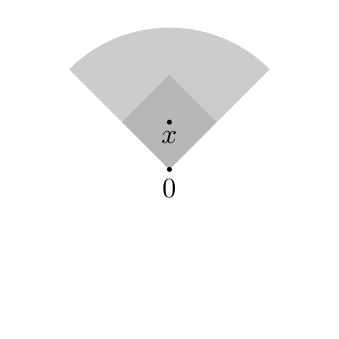
\begin{tikzpicture}[scale=0.6]
		\begin{scope}
			\clip (0,-1) circle (3);
		\fill(0,0) circle (1.5pt);
		\path (0,0) node [below]{$x$};
		\fill[opacity=0.1](1,0)--(0,1)--(-1,0)--(0,-1)--cycle;
		\fill (0,-1) circle (1.5pt);
		\path (0,-1) node [below]{$0$};
		\fill[opacity=0.2] (0,-1)--(4,3)--(0,4)--(-4,3)--cycle;
		\end{scope}
		\end{tikzpicture}
	\end{minipage}
	\begin{minipage}{0.45\linewidth}
		\centering
	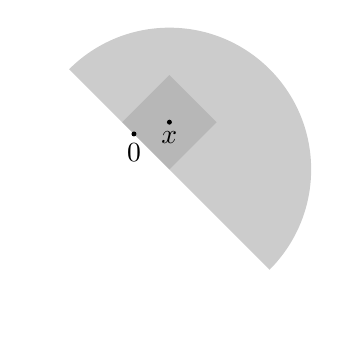
\begin{tikzpicture}[scale=0.6]
		\begin{scope}
			\clip (0,-1) circle (3);
		\fill(0,0) circle (1.5pt);
		\path (0,0) node [below]{$x$};
		\fill[opacity=0.1](1,0)--(0,1)--(-1,0)--(0,-1)--cycle;
		\fill (-0.75,-0.25) circle (1.5pt);
		\path (-0.75,-0.25) node [below]{$0$};
		\fill[opacity=0.2] (-4,3)--(4,-5)--(8,-1)--(0,7)--cycle;
		\end{scope}
		\end{tikzpicture}
	\end{minipage}

\end{frame}

\begin{frame}
\begin{Satzz}
	{(Theorem 4.35 in the book)}{} Let \(A\in \RR^{m\times N }\) and \(x\in \RR^N \). Then
	\[
	\left.\begin{array}{c}

		x\text{ is the unique minimizer} \\  \text{of }
		\left\{\|z\|_1\,\big|\, Az=Ax\right\}
	\end{array}\right\} \iff \ker(A)\cap T(x)=\{0\}\,.
	\]
\end{Satzz}
\end{frame}

\begin{frame}
	\begin{Satzz}
{(Theorem 4.36 in the book)}{} Let \(A\in \RR^{m\times N}\), \(x\in \RR^N\) and \(e\in \RR^m \) such that \(\|e\|_2\le \eta\). Assume
\[\exists \tau>0:\;\;\inf_{v\in T(x)\cap \pp B_1^{\|\cdot\|_2}}\|Av\|_2\ge \tau\,.\]
Then, if \(x^{\#}\) is a minimizer of the problem
\[\min\left\{\|z\|_1\,\big|\,z\in \RR^N,\;\;\|Az-(Ax+e)\|_2\le \eta\right\}\,,\]
we have that
\[\|x-x^{\#}\|_2\le \frac{2\eta}{\tau}\,.\]
	\end{Satzz}	
\end{frame}

\end{document}